\documentclass[master=cws,masteroption=gs]{kulemt}

\setup{title={Automatisch uitrol van SQL systemen en vergelijking van beschikbaarheid},
  author={Thomas Uyttendaele},
  promotor={Prof.\,dr.\,ir.\ Wouter Joosen},
  assessor={Ir.},
  assistant={Ir.\ B. Vanbrabant}}
% De volgende \setup mag verwijderd worden als geen fiche gewenst is.
\setup{filingcard,
  translatedtitle={Automatisch uitrol van SQL systemen en vergelijking van beschikbaarheid},
  udc=621.3,
  shortabstract={Hier komt een heel bondig abstract van hooguit 500
      woorden. \LaTeX\ commando's mogen hier gebruikt worden. Blanco lijnen
   (of het commando \texttt{\string\pa r}) zijn wel niet
   toegelaten!
  \endgraf \lipsum[2]}}
% Verwijder de "%" op de volgende lijn als je de kaft wil afdrukken
%\setup{coverpageonly}
% Verwijder de "%" op de volgende lijn als je enkel de eerste pagina's wil
% afdrukken en de rest bv. via Word aanmaken.
%\setup{frontpagesonly}

% Kies de fonts voor de gewone tekst, bv. Latin Modern
\setup{font=lm}

% Hier kun je dan nog andere pakketten laden of eigen definities voorzien

% Tenslotte wordt hyperref gebruikt voor pdf bestanden.
% Dit mag verwijderd worden voor de af te drukken versie.
\usepackage[pdfusetitle,colorlinks,plainpages=false]{hyperref}
\usepackage[dutch]{babel}
\usepackage{lipsum} % for dummy text only
\usepackage{todonotes}
\usepackage[acronym]{glossaries}
\newglossaryentry{eventualconsistency}{
	name=eventuele consistentie,
	description= aaa
}

\newglossaryentry{rangequery}{
	name=range query,
	plural= range queries,
	description= Het opvragen van een set van records met behulp van een enkele query
}

\newglossaryentry{base}{
	name=BASE,
	description= aaa
}
\newglossaryentry{acid}{
	name=ACID,
	description= aaa
}

\newglossaryentry{nosql}{
	name=NoSQL,
	description= aaa
}

\newglossaryentry{horizontaalschaalbaar}{
	name=horizontaal schaalbaar,
	description= aaa
}

\newglossaryentry{yum}{
	name=yum,
	description= aaa
}

\newglossaryentry{apt-get}{
	name=apt-get,
	description= aaa
}

\newglossaryentry{CAP}{
	name=CAP,
	description= aaa
}

\newglossaryentry{IMP}{
	name=IMP,
	description= aaa
}

\newglossaryentry{DBMS}{
	name=DBMS,
	plural= DBMS's,
	description= aaa
}

\newglossaryentry{HDFS}{
	name=HDFS,
	description= Hadoop Distributed File System
}

\newglossaryentry{eventsupport}{
	name=event support,
	description= a
}

\makeglossaries
%%%%%%%
% Om wat tekst te genereren wordt hier het lipsum pakket gebruikt.
% Bij een echte masterproef heb je dit natuurlijk nooit nodig!
\IfFileExists{lipsum.sty}%
 {\usepackage{lipsum}\setlipsumdefault{11-13}}%
 {\newcommand{\lipsum}[1][11-13]{\par Hier komt wat tekst: lipsum ##1.\par}}
%%%%%%%

%\includeonly{hfdst-n}
\begin{document}

\begin{preface}
\todo{Voorwoord schrijven}
\lipsum
  
\end{preface}

\tableofcontents*
\listoftodos
\begin{abstract}
\todo{Abstract schrijven}

  In dit \texttt{abstract} environment wordt een al dan niet uitgebreide
  samenvatting van het werk gegeven. De bedoeling is wel dat dit tot
  1~bladzijde beperkt blijft.
  \lipsum
\end{abstract}

% Een lijst van figuren en tabellen is optioneel
%\listoffigures
%\listoftables
% Bij een beperkt aantal figuren en tabellen gebruik je liever het volgende:
\listoffiguresandtables
% De lijst van symbolen is eveneens optioneel.
% Deze lijst moet wel manueel aangemaakt worden, bv. als volgt:
\chapter{Lijst van afkortingen en symbolen}
\section*{Afkortingen}
\begin{flushleft}
  \renewcommand{\arraystretch}{1.1}
  \begin{tabularx}{\textwidth}{@{}p{12mm}X@{}}
    IMP   & Infrastructure Management Platform \\
    DBMS   & Databasemanagementsysteem \\
  \end{tabularx}
\end{flushleft}
\section*{Symbolen}
\begin{flushleft}
  \renewcommand{\arraystretch}{1.1}
  \begin{tabularx}{\textwidth}{@{}p{12mm}X@{}}
    42    & aaa \\
  \end{tabularx}
\end{flushleft}

% Nu begint de eigenlijke tekst
\mainmatter

\chapter{Inleiding}
\label{inleiding}
In dit hoofdstuk wordt het werk ingeleid. Het doel wordt gedefinieerd en er
wordt uitgelegd wat de te volgen weg is (beter bekend als de rode draad).

\todo{Schrijf inleiding}

%%% Local Variables: 
%%% mode: latex
%%% TeX-master: "masterproef"
%%% End: 

\chapter{Probleem- en doelstelling}

\section{Probleemstelling}
Sinds het begin van WEB 2.0 is het gebruik van het internet veranderd, van een statisch tot een dynamische omgeving waar iedereen een persoonlijke en individuele ervaring heeft. Samen met deze evolutie is ook het type, de hoeveelheid en het gebruik van data en de opslag ervan veranderd. 

\paragraph{}
Deze verandering kan allereerst toegeschreven worden aan de toename in het aantal website, daarnaast is ook de content van een webpagina veranderd, geen statische pagina's met enkel tekst maar ook afbeeldingen en (korte) videofragmenten zijn aanwezig. Deze content wordt ook niet meer enkel door de websitebeheerder online geplaatst maar de gebruikers kunnen zelf hun data invoegen en krijgen gepersonaliseerde en dynamische pagina's te zien. 
Tenslotte is ook de toename in het aantal gebruikers, op 30 juni 2012 waren er meer als 2.4 miljard gebruikers van het internet, een toename van meer als 500\% op 12 jaar tijd.  
\cite{WorldInternetStatics}

\paragraph{}
Al deze veranderingen hebben ook hun doorslag op de achterliggende infrastructuur. Waar kleinere en statische websites nog konden gehost worden op een enkele server, is dit niet meer het geval voor hedendaagse (populaire) websites. 
Een onderdeel van deze web applicaties is de databases waarin de vereiste data kan in worden opgeslagen worden en later opgevraagd worden. Veel van deze databases zijn ontworpen naar het systeem van de relationele databases, uitgewerkt naar Codd \cite{Codd:1970:RMD:362384.362685}.

Voor talrijke van de huidige applicaties is de voorwaarden voor dataopslag verschillend met deze van de jaren 70. Enkele systemen hebben geen nood meer aan onmiddellijke consistentie maar hebben genoeg aan \gls{eventualconsistency}. Onder andere omwille van deze reden is er een stroming van nieuwe database systemen gekomen genaamd \gls{nosql}. Onder deze noemer vallen vele systemen, elk eigen in hun soort en aangepast aan bepaalde manieren van dataopslag en de daarvoor nodige vereisten, een belangrijk element is het \gls{horizontaalschaalbaar} zijn van deze systemen. Met andere woorden, deze databases zijn ontworpen om de data over meerdere systemen te verspreiden om de load te verspreiden. 

\paragraph{}
\Gls{horizontaalschaalbaar} brengt verschillende voordelen mee, maar zorgt ook voor 2 problemen die in deze thesis zullen aanbod komen, namelijke de uitrol en daarnaast wat de implicaties zijn van een gedistribueerd datasysteem. 

\subsection{Uitrollen van gedistribueerde databases}
Voor geavanceerde toepassingen is het gebruik van gespecialiseerde en/of gedistribueerde databases een noodzaak. Maar de tijdsduur van de beslissing dat dit het geval is tot een werkende omgeving hebben, is niet te onderschatten en dit omwille van verschillende componenten. 

\paragraph{}Een eerste stap die doorlopen wordt, is het opzoeken van de nodige informatie over de verschillende databases, nu bestaan er al verschillende websites en papers waar informatie opgezocht kan worden, maar een consistente test bestaat niet. Een voorbeeld van een vergelijkingswebsite is bijvoorbeeld vsChart \cite{vsChart}, ook verschillende papers brengen vergelijkingen naar voor in onder andere performantie en de verschillende data modellen. Maar in de meeste gevallen blijft het aangeraden om de informatie op te zoeken op de website van de software zelf, deze evolueert snel en informatie van een jaar oud kan al verouderd zijn en zo incorrect. 

Al deze informatie zou de ontwikkelaar een mogelijkheid geven om de verschillende systemen te kunnen vergelijken en een keuze te maken met welke database hij verder wenst te gaan. 

\paragraph{} Na de selectie van een specifieke database, komt de keuze voor de opstelling van de database. Bepaalde databases hebben ondersteuning voor Master-slave, andere hebben ondersteuning voor sharding en nog andere hebben een combinatie van de twee. Deze verschillende manieren zorgt ervoor dat er geen eenduidige manier is om alle verschillende systemen consequent uit te rollen. De ontwikkelaar zal in deze stap een opstellen kiezen onder welke hij de database zal uitrollen. 

\paragraph{} Nu de databasesoftware en de opstelling is gekozen, kunnen de verschillende machines fysiek opgesteld worden. Dit wil zeggen, de opstellening wordt fysiek opgesteld: de computers kiezen, deze op de juiste locatie zetten en te verbinden. De meeste \gls{nosql} systemen zijn ontworpen om te draaien op commodity hardware wat wil zeggen dat gewone consumenten computers volstaan. 

\paragraph{} In het volgend stadium, komt de softwarematige installatie: beginnende bij het besturingssysteem tot de database software zelf. De meeste van deze databases draaien onder verschillende Linux versies. De meeste hebben wel de nodige andere software nodig om ook te kunnen draaien, een voorbeeld is HBase dat Java en Hadoop nodig heeft. 

Deze systemen worden geïnstalleerd en nadien geconfigureerd. Waar voor de installatie meestal nog standaard tools zoals \gls{yum} of \gls{apt-get} gebruikt kunnen worden, is de configuratie afhankelijk van systeem tot systeem. Bepaalde systemen zoals Pgpool werken volledig met configuratie bestanden, andere systemen zoals MongoDB werken voornamelijk met een configuratie via de shell, nog andere, zoals HBase, hebben een basis configuratie waarbij men zich aanmeldt bij een node en daar de rest van de configuratie ontvangen. Deze verschillende aanpakken maken het opzetten van verschillende systemen niet eenvoudiger.

\paragraph{} Nu het systeem draait, kan het systeem getest worden en bekeken worden of het voldoet aan de vooropgesteld benodigdheden. Indien dit niet het geval is, kan een aanpassing aan de opstelling misschien voldoen of dient een ander systeem geselecteerd worden. 

Vervolgens kan de ontwerpen verder gaan met het ontwerpen van de applicatie, waar de databaselaag uiteindelijk maar een gedeelte van is. 

Daarnaast zou het kunnen dat de set-up voldoet tijdens het ontwerpen maar niet tijdens de uiteindelijke ingebruikname of maakt de applicatie een groei mee waardoor er extra resources nodig zijn. Nu zijn veel van de databases en zeker de \gls{nosql} databases geschreven om eenvoudig \gls{horizontaalschaalbaar} te zijn: het toevoegen of verwijderen van systemen kan in veel gevallen zelfs dynamisch. 

Deze stappen zijn allemaal niet zo onlogisch maar vragen wel tijd en kennis van de installatie en configuratie van deze systemen. Bij veel lokale systemen wordt de installatie en configuratie automatisch gedaan door onder andere gebruik te maken van \gls{yum} of \gls{apt-get} waarna deze systemen volledig werken, want uiteindelijk dient een ontwerper om nieuwe systemen te ontwikkelen, oa. door het samenbrengen van verschillende componenten die als een black block kunnen beschouwd worden met zo weinig mogelijk configuratie. 

\subsection{Implicatie van gedistribueerde datasystemen}
Een tweede element van de thesis is het onderzoek naar de implicaties van gedistribueerde datasystemen. In dit gebied is er al veel onderzoek gedaan naar de verschillen in datamodellen en performantie maar er is nog geen gerelateerd onderzoek naar de implicaties op de beschikbaarheid van de data. 

\paragraph{}De CAP-theorie van E. Brewer\cite{Brewer:2000:TRD:343477.343502} staat voor consistency, availability en partition tolerance. De volgende definities zoals geformuleerd in \cite{Strauch.NoSQL}:


\textbf{Consistency} of consistentie betekent dat na een aanpassing van een schrijver in een gedeelte databron, alle lezers deze aanpassing zien. 

\textbf{Availability} of beschikbaarheid, meer bepaald hoge beschikbaarheid, betekent dat een systeem de mogelijkheid heeft om verdere operaties (lezen en/of schrijven) te verwerken indien een of meerdere nodes in de cluster niet beschikbaar zijn.

\textbf{Partition toleranc}e of partitie tolerantie betekent dat het systeem verder kan blijven werken in zijn geheel indien de volledige cluster (tijdelijke of finaal) in twee of meer delen opgedeeld is. Een andere betekenis is dat er de mogelijkheid is tot het dynamisch verwijderen of toevoegen van nodes, waarbij de te verwijderen of toe te voegen nodes bezien worden als een eigen netwerk partitie. 

\paragraph{} Vervolgens stelt E. Brewer dat in een systeem met gedeelde data maximaal aan 2 van de 3 elementen van de CAP-theorie kan voldaan worden. 

Dit heeft invloed op de beschikbaarheid van de data in gedistribueerde databases, maar verschillende database systemen kiezen verschillende beschikbaarheden. Bepaalde database systemen geven geen consistentie maar enkel eventuele consistentie waarbij de aanpassing na verloop van tijd maar beschikbaar is voor alle gebruikers. Indien een ontwerper hier geen rekening bij houdt bij de implementatie, kunnen in reservatiesysteem bijvoorbeeld dubbele boekingen voorkomen over de tijd. 

\section{Doelstelling}
De doelstellingen voor deze thesis bestaat uit 2 delen, net zoals de probleemstelling. In eerste instantie de uitrol van gedistribueerde databases, in tweede instantie de implicaties op de beschikbaarheid van de data. 

\subsection{Uitrol van gedistribueerde databases}
Het eerste gedeelte van de doelstellingen is gerelateerd met de uitrol van gedistribueerde databases, voornamelijk het vereenvoudigen van de uitrol. 

Net zoals \gls{yum} en \gls{apt-get} de mogelijkheid geven om lokaal op een eenvoudige manier software te installeren, zal in deze thesis de uitrol van verschillende database systemen geautomatiseerd worden en dit door middel van \gls{IDP}. 

Aangezien er geen unieke opstelling is, zal er nog steeds een configuratie nodig zijn. Maar het doel is om deze configuratie eenvoudiger te maken op basis van een model. 

De gebruiker zal enkel een systeem moeten selecteren, de set-up bepalen en de systemen fysiek opstellen. De softwarematige installatie en configuratie zal niet langer door gebruiker moeten gebeuren maar bepaalde componenten toewijzen aan bepaalde machines, met de nodige relaties tussen de componenten. 

\subsection{Implicatie op beschikbaarheid van gedistribueerde datasystemen} 
Naast de automatisatie van de uitrol, zal er ook gefocust worden op het testen van deze systemen. Dit niet op basis van de performantie maar dit op de beschikbaarheid van de data. 

Zoals vermeldt in de probleemstelling, hebben verschillende database systemen een ander methode om om te gaan met het niet beschikbaar zijn van een node en netwerk partities. 

Om deze verschillen te vergelijken zullen er testen geschreven worden om de keuzes en hun implicaties duidelijk te maken. 

Tenslotte zullen deze testen ook beschikbaar gesteld worden om op een eenvoudige manier ook op andere systemen uitgerold te worden en verificatie van de data mogelijk te maken. Daarnaast is het zo ook mogelijk om deze testen opnieuw uit te voeren indien er updates beschikbaar komen, die mogelijke verbeteringen brengen. 

\chapter{Automatisch uitrollen van databases}
\section{Inleiding}
%Inleiding

\section{IMP: Framework voor installatie}
%Uitleg van IMP
\todo{Te schrijven}
%Uitleg van hoe voor elk systeem

\section{MongoDB}
In deze sectie zal 

\subsection{Werking van MongoDB}
MongoDB heeft gekozen om bij gedistribueerde database op te splitsen in 2 keuzes, een eerste is door middel van \textit{replicaset}s en daarnaast door middel van \textit{shard}ing. 

\paragraph{}Bij \textit{replicaset} is een master-slave configuratie van de MongoDB nodes, met de master benoemd als primary en de slaves als secondary (figuur \ref{fig:mongodb-replicaset}). De data is nog steeds beschikbaar zolang meer als de helft van de nodes beschikbaar zijn. De schrijfoperaties worden eerst naar de primary gestuurd en vervolgens door MongoDB naar de secondaries gesynchroniseerd. Ook leesoperaties worden standaard enkel naar de primary gestuurd maar dit kan aangepast worden in de configuratie. 

Met behulp van een heartbeat houden wordt de status van de verschillende nodes opgevraagd elke 10 seconden en indien de primary niet meer beschikbaar is zal een secondary gestemd worden tot primary (figuur \ref{fig:mongodb-replicaset-vote}). 

\begin{figure}[!htb]
	    \centering
    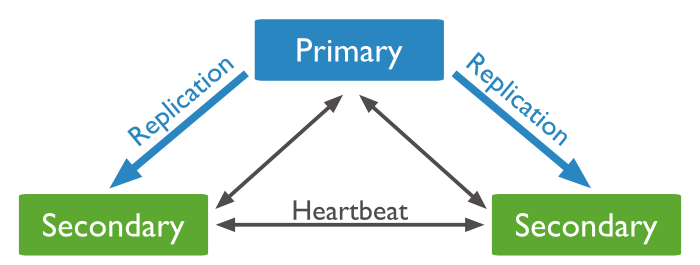
\includegraphics[width=0.7\textwidth]{img/mongodb-replica-set-primary-with-two-secondaries.png}
    \caption{MongoDB: Drie leden van een replicaset met 1 master en 2 slaves. \cite{mongodb-replicaset}}
    \label{fig:mongodb-replicaset}
\end{figure}

\begin{figure}[!htb]
	    \centering
    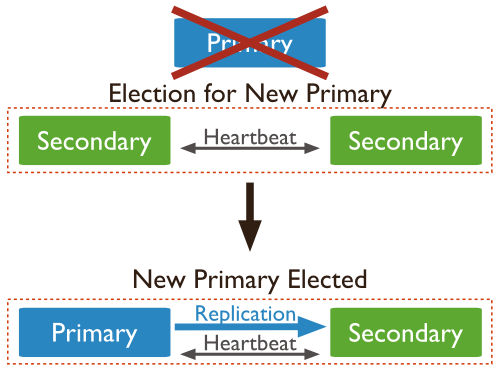
\includegraphics[width=0.7\textwidth]{img/mongodb-replica-set-trigger-election.png}
    \caption{MongoDB: Drie leden van een replicaset met 1 master en 2 slaves. \cite{mongodb-replicaset}}
    \label{fig:mongodb-replicaset-vote}
\end{figure}

\paragraph{} Vervolgens wordt met behulp van \textit{sharding} de data verdeeld over verschillende shards. In productie omgeving wordt aangeraden om een replicaset te nemen als shard maar het is ook mogelijk om een enkele node toe te voegen. 

Voor lees- en schrijfoperaties wordt er hier connectie gemaakt met mongos, dit zijn router nodes die de query naar de nodige shards stuurt. De configuratie van de shards wordt opgeslagen in 1 of 3 configuratie nodes (figuur \ref{fig:mongodb-shards}). 

\begin{figure}[!htb]
	    \centering
    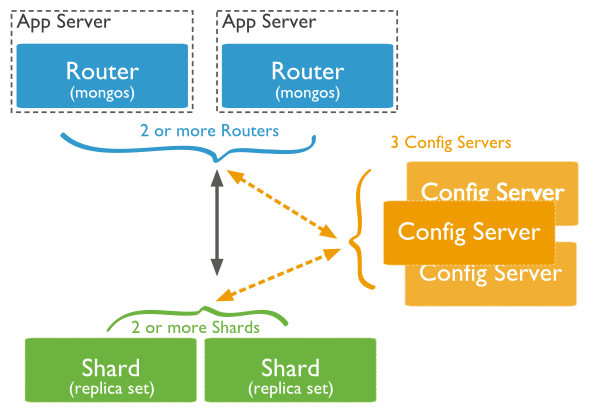
\includegraphics[width=\textwidth]{img/mongo-sharded-cluster-production-architecture.png}
    \caption{MongoDB: Een voorbeeld cluster voor productie met 2 mongos, 3 shards en 3 configuratie servers. \cite{mongodb-shard}}
    \label{fig:mongodb-shards}
\end{figure}

De data wordt verdeeld over de verschillende shards met een door de gebruiker gedefinieerde formule, dit kan door middel van hashing of door het opsplitsen van een waarde in verschillende domeinen. 

\paragraph{} De configuratie van MongoDB is opgesplitst in 2 delen, een configuratiebestand en met behulp van de shell. Als eerste stelt men een configuratiebestand op die aan de instantie basisinformatie meegeeft zoals op welke poort, waar de database op het bestandssysteem op te slaan en welk type de instantie is (enkele node, deel van replicaset, configuratie server of een mongos). 

Het opzetten van de replicasets en sharding verloopt via de shell, met behulp van een commando op een instantie die een deel is van de replicaset kan de replicaset opgezet worden. 
Sharding wordt opgezet door connectie te maken met een mongos en ook hier via commando shards toe te voegen, collecties aan te maken en collecties te verdelen onder shards.

Belangrijk bij sharding is dat bij het opstarten van een mongos al de verschillende configuratie servers meegegeven moeten worden, dit is de enige parameter die meegegeven moet worden in de configuratiebestanden die afhankelijk is van andere instanties. 

\subsection{Uitwerking}


\begin{figure}[!htb]
	    \centering
    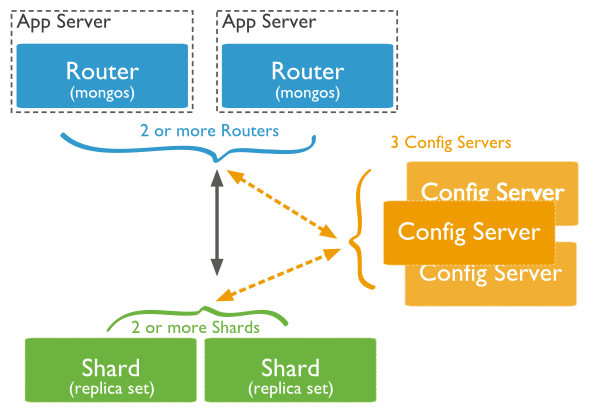
\includegraphics[width=\textwidth]{img/mongo-sharded-cluster-production-architecture.png}
    \caption{MongoDB: Een voorbeeld cluster voor productie met 2 mongos, 3 shards en 3 configuratie servers. \cite{mongodb-shard}}
    \label{fig:mongodb-shards}
\end{figure}
\subsection{Resultaat}
%\chapter{Een volgend hoofdstuk}
\label{hoofdstuk:2}
Een hoofdstuk behandelt een samenhangend geheel dat min of meer op zichzelf
staat. Het is dan ook logisch dat het begint met een inleiding, namelijk
het gedeelte van de tekst dat je nu aan het lezen bent.

\section{Eerste onderwerp in dit hoofdstuk}
De inleidende informatie van dit onderwerp.

\subsection{Een item}
Een tekst staat nooit alleen. Dit wil zeggen dat er zeker ook referenties
nodig zijn. Dit kan zowel naar on-line documenten\cite{wiki} als naar
boeken\cite{pratchett06:_good_omens}.

\section{Figuren}
Figuren worden gebruikt om illustraties toe te voegen. Dit is dan ook de
manier om beeldmateriaal toe te voegen zoals getoond wordt in
figuur~\ref{fig:logo}.

\begin{figure}
  \centering
  
\includegraphics{logokul}
  \caption{Het KU~Leuven logo.}
  \label{fig:logo}
\end{figure}

\section{Tabellen}
Tabellen kunnen gebruikt worden om informatie op een overzichtelijke te
groeperen. Een tabel is echter geen rekenblad! Vergelijk maar eens
tabel~\ref{tab:verkeerd} en tabel~\ref{tab:juist}. Welke tabel vind jij het
duidelijkst?

\begin{table}
  \centering
  \begin{tabular}{||l|lr||} \hline
    gnats     & gram      & \$13.65 \\ \cline{2-3}
              & each      & .01 \\ \hline
    gnu       & stuffed   & 92.50 \\ \cline{1-1} \cline{3-3}
    emu       &           & 33.33 \\ \hline
    armadillo & frozen    & 8.99 \\ \hline
  \end{tabular}
  \caption{Een tabel zoals het niet moet.}
  \label{tab:verkeerd}
\end{table}

\begin{table}
  \centering
  \begin{tabular}{@{}llr@{}} \toprule
    \multicolumn{2}{c}{Item} \\ \cmidrule(r){1-2}
    Animal    & Description & Price (\$)\\ \midrule
    Gnat      & per gram    & 13.65 \\
              & each        & 0.01 \\
    Gnu       & stuffed     & 92.50 \\
    Emu       & stuffed     & 33.33 \\
    Armadillo & frozen      & 8.99 \\ \bottomrule
  \end{tabular}
  \caption{Een tabel zoals het beter is.}
  \label{tab:juist}
\end{table}

\section{Lorem ipsum}
Tenslotte gaan we hier nog wat tekst voorzien zodat er minstens een
bijkomende bladzijde aangemaakt wordt. Dat geeft de gelegenheid om eens te
zien hoe de koptekst en de voettekst zich gedragen.

\subsection{Lorem ipsum dolor sit amet, consectetur adipiscing elit}
Sed nec tortor id felis tristique sodales. Nulla nec massa eu dui fermentum
tincidunt. Integer ullamcorper ante eget eros posuere faucibus. Nam id
ligula ut augue pulvinar vulputate id at purus. Aenean condimentum tortor
eu mi placerat eget eleifend massa mollis. Nam est mi, sagittis quis
euismod eget, sagittis in nibh. Proin elit turpis, aliquam et imperdiet
sed, volutpat eu turpis.

Pellentesque vel enim tellus, vitae egestas turpis. Praesent malesuada elit
non nisi sollicitudin non blandit lacus tincidunt. Morbi blandit urna at
lectus ornare laoreet. Suspendisse turpis diam, lobortis dictum luctus
quis, commodo at lorem. Integer lacinia convallis ultricies. Sed quis augue
neque, eu malesuada arcu. Nullam vehicula, purus vitae sagittis pulvinar,
erat eros semper massa, eu egestas nibh erat quis magna. Cras pellentesque,
nisl eu dapibus volutpat, urna augue ornare quam, quis egestas lectus nulla
a lectus.

Vivamus dictum libero in massa cursus sed vulputate eros imperdiet. Donec
lacinia, libero ac lobortis egestas, nibh dui ornare arcu, luctus porttitor
velit massa sit amet quam. Maecenas scelerisque laoreet diam, vitae congue
quam adipiscing vitae. Aliquam cursus nisl a leo convallis eleifend
fermentum massa porta. Nunc libero quam, dapibus dapibus molestie sit amet,
faucibus vel nunc.

\subsection{Praesent auctor venenatis posuere}
Sed tellus augue, molestie in pulvinar lacinia, dapibus non ipsum. Fusce
vitae mi vitae enim ullamcorper hendrerit eu malesuada est. Proin iaculis
ante sed nibh tincidunt vel interdum libero posuere. Vivamus accumsan metus
quis felis congue suscipit dapibus enim mattis. Fusce mattis tortor eget
ipsum interdum sagittis auctor id metus.

Integer diam lacus, pharetra sit amet tempor et, tristique non lorem.
Aenean auctor, nisi eu interdum fermentum, lectus massa adipiscing elit,
sed facilisis orci odio a lectus. Proin mi nibh, tempus quis porta a,
viverra quis enim. In sollicitudin egestas libero, quis viverra velit
molestie eget. Nulla rhoncus, dolor a mollis vestibulum, lacus elit semper
nisi, nec sollicitudin sem urna eu magna. Nunc sed est urna, euismod congue
mi.

\subsection{Cras vulputate ultricies venenatis}
Vivamus eros urna, sodales accumsan semper vel, lobortis sit amet mauris.
Etiam condimentum eleifend lorem, ullamcorper ornare lectus aliquet vitae.
Praesent massa enim, interdum sit amet semper et, venenatis ut elit.
Quisque faucibus, quam ac lacinia imperdiet, nulla neque elementum purus,
tempus rutrum justo massa porta sapien. Vestibulum ante ipsum primis in
faucibus orci luctus et ultrices posuere cubilia Curae; Sed ultrices
interdum mi, et rhoncus sapien rutrum sed.

Duis elit orci, molestie quis sollicitudin sed, convallis non ante.
Maecenas tincidunt condimentum justo, et ultricies leo tristique vitae.
Vestibulum quis quam non lectus dapibus eleifend a vitae nibh. Nam nibh
justo, pharetra quis iaculis consequat, elementum quis justo. Etiam mollis
lacinia lacus, nec sollicitudin urna lobortis ac. Nulla facilisi.

Proin placerat risus eleifend erat ultricies placerat. Etiam rutrum magna
nec turpis euismod consectetur. Phasellus tortor odio, lacinia imperdiet
condimentum sed, faucibus commodo erat. Phasellus sed felis id ante
placerat ultrices. Aenean tempor justo in tortor volutpat eu auctor dolor
mollis. Aenean sit amet risus urna. Morbi viverra vehicula cursus.

\subsection{Donec nibh ante, consectetur et posuere id, tempus nec arcu}
Curabitur a tellus aliquet ipsum pellentesque scelerisque. Etiam congue,
risus et volutpat rutrum, est purus dapibus leo, non cursus metus felis
eget ligula. Vivamus facilisis tristique turpis, ut pretium lectus luctus
eleifend. Fusce magna sapien, ullamcorper vitae fringilla id, euismod quis
ante.

Phasellus volutpat, nunc et pharetra semper, sem justo adipiscing mauris,
id blandit magna quam et orci. Vestibulum a erat purus, ut molestie ante.
Vestibulum ante ipsum primis in faucibus orci luctus et ultrices posuere
cubilia Curae; Proin turpis diam, consequat ut ullamcorper ut, consequat eu
orci. Sed metus risus, fringilla nec interdum vel, interdum eu nunc.
Suspendisse vel sapien orci.

\subsection{Morbi et mauris tempus purus ornare vehicula}
Mauris sit amet diam quam, eget luctus purus. Sed faucibus, risus semper
eleifend iaculis, mi turpis bibendum nisl, quis cursus nibh nisl sit amet
ipsum. Vestibulum tempor urna vitae mi auctor malesuada eget non ligula.
Nullam convallis, diam vel ultrices auctor, eros eros egestas elit, sed
accumsan arcu tortor eget leo. Vestibulum orci purus, porttitor in pharetra
eget, tincidunt eget nisl. Nullam sit amet nulla dui, facilisis vestibulum
dui.

Donec faucibus facilisis mauris ac cursus. Duis rhoncus quam sed nisi
laoreet eu scelerisque massa tincidunt. Vivamus sit amet libero nec arcu
imperdiet tempor quis non libero. Sed consequat dignissim justo. Phasellus
ullamcorper, velit quis posuere vulputate, felis erat tincidunt mauris, at
vestibulum justo lectus et turpis. Maecenas lacinia convallis euismod.
Quisque egestas fermentum sapien eu dictum. Sed nec lacus in purus dictum
consequat quis vel nisl. Fusce non urna sem. Curabitur eu diam vitae elit
accumsan blandit. Nullam fermentum nunc et leo dictum laoreet. Donec semper
varius velit vel fringilla. Vivamus eu orci nunc.

\section{Besluit van dit hoofdstuk}
Als je in dit hoofdstuk tot belangrijke resultaten of besluiten gekomen
bent, dan is het ook logisch om het hoofdstuk af te ronden met een
overzicht ervan. Voor hoofdstukken zoals de inleiding en het
literatuuroverzicht is dit niet strikt nodig.

%%% Local Variables: 
%%% mode: latex
%%% TeX-master: "masterproef"
%%% End: 

% ... en zo verder tot
%\chapter{Het laatste hoofdstuk}
\label{hoofdstuk:n}
Een hoofdstuk behandelt een samenhangend geheel dat min of meer op zichzelf
staat. Het is dan ook logisch dat het begint met een inleiding, namelijk
het gedeelte van de tekst dat je nu aan het lezen bent.

\section{Eerste onderwerp in dit hoofdstuk}
De inleidende informatie van dit onderwerp.

\subsection{Een item}
De bijbehorende tekst. Denk eraan om de paragrafen lang genoeg te maken en
de zinnen niet te lang.

Een paragraaf omvat een gedachtengang en bevat dus steeds een paar zinnen.
Een paragraaf die maar \'e\'en lijn lang is, is dus uit den boze.

\section{Tweede onderwerp in dit hoofdstuk}
Er zijn in een hoofdstuk verschillende onderwerpen. We zullen nu
veronderstellen dat dit het laatste onderwerp is.

\section{Besluit van dit hoofdstuk}
Als je in dit hoofdstuk tot belangrijke resultaten of besluiten gekomen
bent, dan is het ook logisch om het hoofdstuk af te ronden met een
overzicht ervan. Voor hoofdstukken zoals de inleiding en het
literatuuroverzicht is dit niet strikt nodig.

%%% Local Variables: 
%%% mode: latex
%%% TeX-master: "masterproef"
%%% End: 

\chapter{Besluit}
\label{besluit}
De masterproeftekst wordt afgesloten met een hoofdstuk waarin alle
besluiten nog eens samengevat worden. Dit is ook de plaats voor suggesties
naar het verder gebruik van de resultaten, zowel industri"ele toepassingen
als verder onderzoek.

%%% Local Variables: 
%%% mode: latex
%%% TeX-master: "masterproef"
%%% End: 


% Indien er bijlagen zijn:
\appendixpage*          % indien gewenst
\appendix
%\chapter{De eerste bijlage}
\label{app:A}
In de bijlagen vindt men de data terug die nuttig kunnen zijn voor de
lezer, maar die niet essentieel zijn om het betoog in de normale tekst te
kunnen volgen. Voorbeelden hiervan zijn bronbestanden,
configuratie-informatie, langdradige wiskundige afleidingen, enz.

In een bijlage kunnen natuurlijk ook verdere onderverdelingen voorkomen,
evenals figuren en referenties\cite{h2g2}.

\section{Meer lorem}
\lipsum[50]

\subsection{Lorem 15--17}
\lipsum[15-17]

\subsection{Lorem 18--19}
\lipsum[18-19]

\section{Lorem 51}
\lipsum[51]

%%% Local Variables: 
%%% mode: latex
%%% TeX-master: "masterproef"
%%% End: 

% ... en zo verder tot
%\chapter{De laatste bijlage}
\label{app:n}
In de bijlagen vindt men de data terug die nuttig kunnen zijn voor de
lezer, maar die niet essentieel zijn om het betoog in de normale tekst te
kunnen volgen. Voorbeelden hiervan zijn bronbestanden,
configuratie-informatie, langdradige wiskundige afleidingen, enz.

\section{Lorem 20-24}
\lipsum[20-24]

\section{Lorem 25-27}
\lipsum[25-27]

%%% Local Variables: 
%%% mode: latex
%%% TeX-master: "masterproef"
%%% End: 


\backmatter
% Na de bijlagen plaatst men nog de bibliografie.
% Je kan de  standaard "abbrv" bibliografiestijl vervangen door een andere.
\printglossary
\bibliographystyle{abbrv}
\bibliography{overige/referenties}

\end{document}

%%% Local Variables: 
%%% mode: latex
%%% TeX-master: t
%%% End: 
